\chapter{Specifications} \label{specifications}

\section{Functional Description} \label{functional-description}

The Roa Logic APB4 Multiplexer is a highly configurable, fully parameterized
soft IP to enable a single APB4 based Master (Host) to communicate with
multiple APB4 Slaves (Peripherals). It is fully compliant with the
\emph{AMBA APB v2.0} bus protocols.

The IP contains a single Master Interface to connect to the APB4 Host,
and a user defined number of Slave Interfaces.

The multiplexer functions as follows:

\begin{itemize}
\item
  Transactions on the APB4 Bus are decoded by matching addresses on the
  APB4 address bus to an address map defined by the \texttt{SLV\_ADDR[n]} and
  \texttt{SLV\_MASK[n]} inputs of the multiplexer 
\item
  Communication with a peripheral is enabled by asserting the
  appropriate \texttt{SLV\_PSEL[n]} output signal based on the address
  mapping (See section 4.3.1)
\item
  Peripheral-specific control signals \texttt{SLV\_PSLVERR[n]}and
  \texttt{SLV\_READY[n]}, together with the Read Data Bus signals
  \texttt{SLV\_PRDATA[n]} during a read transaction, are then multiplexed
  back to the Master Interface.
\end{itemize}

\section{Master Interface} \label{master-interface}

The APB4 Multiplexer Master Interface consists of the following subset
of APB4 bus signals:

\begin{itemize}
\item
  \texttt{PADDR} and \texttt{PSEL} inputs to enable address space decoding
\item
  \texttt{PREADY} and \texttt{PSLVERR} outputs derived from the selected peripheral
\item
  \texttt{PRDATA} read data bus output derived from the selected peripheral
  during a read transaction
\end{itemize}

All other APB4 bus signals are connected directly to each peripheral

\section{Slave Interfaces} \label{slave-interfaces}

The APB4 Multiplexer generates a user-defined number (`n') of Slave
Interfaces that consist of the following subset of APB4 bus signals:

\begin{itemize}
\item
  \texttt{PSEL[n]} outputs used to select an individual peripheral during a
  transaction
\item
  \texttt{PREADY[n]} and \texttt{PSLVERR[n]} control signal inputs from each
  peripheral which are multiplexed as outputs on the Master Interface
\item
  \texttt{PRDATA[n]} read data bus inputs from each peripheral which is
  multiplexed to the Master Interface
\end{itemize}

\section{Address Space Configuration} \label{address-space-configuration}

Each Slave Port has an Address Base (\texttt{SLV\_ADDR[n]}) and Address Mask
(\texttt{SLV\_MASK[n]}) port. Together these set the address range covered by
each Slave Port. (See section 4.3.5)

\begin{figure*}[htb]
	\centering
	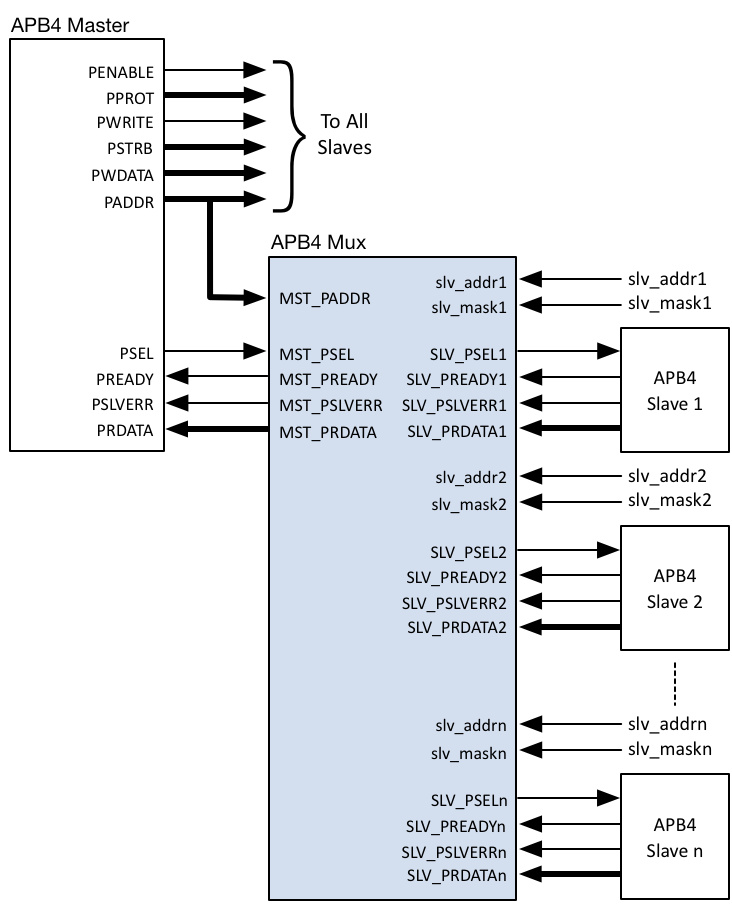
\includegraphics{assets/img/APB4-Mux-Sig}
	\caption{APB4 Multiplexer Signalling}
	\label{fig:apb4-mux-sig}
\end{figure*}

While the Address Base and Address Mask values may be changed dynamically,
assigning static values according to a predefined address map is
typical.
